%----------HEADING-----------------
\begin{minipage}[c]{0.75\textwidth}
\textbf{\huge Davide Chirichella} \\
Luogo: Bologna, Italia \\
Email: \href{mailto:davidechirichella10@gmail.com}{davidechirichella10@gmail.com} \\
GitHub: \href{https://github.com/chirichexe}{github.com/chirichexe} \\
LinkedIn: \href{https://www.linkedin.com/in/davide-chirichella}{linkedin.com/in/davide-chirichella}
\end{minipage}
\begin{minipage}[c]{0.2\textwidth}
\begin{flushright}
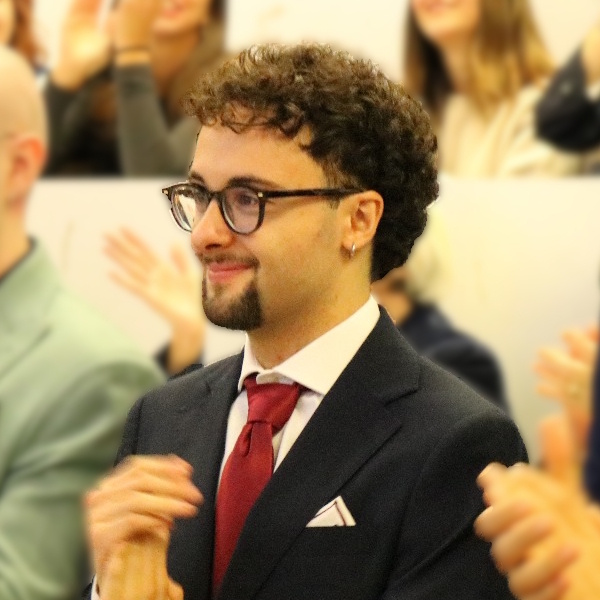
\includegraphics[width=3cm]{picture.jpg}
\end{flushright}
\end{minipage}
\vspace{10pt}


%-----------EDUCATION-----------------
\section{Istruzione}
  \resumeSubHeadingListStart
    \resumeSubheading
      {Alma Mater Studiorum - Università di Bologna}{Bologna, Italia}
      {Laurea Magistrale in Ingegneria Informatica; Media: 29.5/30}{2025 -- In corso}
    \resumeSubheading
      {Università di Stoccolma}{Stoccolma, Svezia}
      {Scambio Erasmus+ --- Computer and Systems Sciences}{Ago 2026 -- Feb 2027}
    \resumeSubheading
      {Alma Mater Studiorum - Università di Bologna}{Bologna, Italia}
      {Laurea Triennale in Ingegneria Informatica; Voto: 107/110}{2022 -- 2025}
      \resumeItemListStart
        \resumeItem{Tesi}{\textit{Analisi delle performance in ambienti Cloud-Edge per IoT}}
      \resumeItemListEnd
    \resumeSubheading
      {Liceo Scientifico Galileo Galilei}{Potenza, Italia}
      {Diploma di Maturità Scientifica}{2017 -- 2022}
  \resumeSubHeadingListEnd


%-----------SKILLS-----------------
\section{Competenze Tecniche}
  \begin{itemize}[leftmargin=*]
    \resumeItem{Container \& Orchestrazione}{Docker, Docker Swarm, Kubernetes, Istio, Crossplane}
    \resumeItem{Infrastruttura \& Automazione}{Linux, Bash, Terraform, Ansible, Vagrant, VirtualBox, CI/CD, GitOps}
    \resumeItem{Osservabilità}{Prometheus, Grafana, OpenTelemetry}
    \resumeItem{Sviluppo \& Database}{React.js, Node.js, C\#, MySQL, MongoDB}
  \end{itemize}


%-----------EXPERIENCE-----------------
\section{Esperienza Lavorativa}
  \resumeSubHeadingListStart

    \resumeSubheading
      {HoDiritto (Startup)}{Ibrido}
      {Junior DevOps Engineer}{Feb 2026 -- In corso}
      \resumeItemListStart
        \resumeItemNoTitle{Realizzazione e gestione dell'infrastruttura a microservizi su Docker Swarm per l'MVP di una startup early-stage, incluse pipeline CI/CD, workflow GitOps, monitoraggio e sicurezza.}
        \resumeItem{Tech Stack}{\textit{Docker, Terraform, MongoDB}}
      \resumeItemListEnd

    \resumeSubheading
      {Alma Mater Studiorum - Università di Bologna}{Bologna, Italia}
      {Tutor Didattico --- Amministrazione di Sistema}{Feb 2026 -- In corso}
      \resumeItemListStart
        \resumeItemNoTitle{Supporto agli studenti della laurea triennale in amministrazione di sistemi Linux, shell scripting e Infrastructure as Code (IaC).}
        \resumeItem{Tech Stack}{\textit{Linux, Bash, VirtualBox, Ansible, Vagrant}}
      \resumeItemListEnd

    \resumeSubheading
      {Mobile Middleware Research Group}{Ibrido}
      {Studente Tirocinante}{Feb 2025 -- Lug 2025}
      \resumeItemListStart
        \resumeItemNoTitle{Progettazione di un'infrastruttura edge-cloud per l'orchestrazione IoT e deploy del relativo stack di monitoraggio.}
        \resumeItemNoTitle{Sviluppo di un Kubernetes Operator per il provisioning automatico dei dispositivi IoT; configurazione di Istio per integrare i microservizi Docker edge nel cluster Kubernetes primario.}
        \resumeItem{Tech Stack}{\textit{Docker, Kubernetes, Istio, Crossplane, Prometheus, Grafana, OpenTelemetry}}
      \resumeItemListEnd

    \resumeSubheading
      {Project Quality Systems S.R.L.}{Remoto}
      {Software Engineer}{2023 -- 2026}
      \resumeItemListStart
        \resumeItemNoTitle{Sviluppo e scalabilità di una piattaforma gestionale aziendale basata su React.js e Node.js con backend MySQL.}
        \resumeItemNoTitle{Manutenzione e ottimizzazione di applicazioni interne legacy scritte in C\#.}
        \resumeItem{Tech Stack}{\textit{React.js, Node.js, MySQL, C\#}}
      \resumeItemListEnd

  \resumeSubHeadingListEnd


%-----------LANGUAGES-----------------
\section{Lingue}
  \begin{itemize}[leftmargin=*]
    \resumeItem{Italiano}{Madrelingua}
    \resumeItem{Inglese}{B2 --- Intermedio Superiore (Cambridge English First, FCE, Giugno 2022)}
  \end{itemize}
